\documentclass[landscape]{article}
\usepackage[dvipsnames]{xcolor}
\usepackage{tikz}

\usetikzlibrary{patterns,snakes}
\usepackage{stackengine}

\begin{document}


\begin{center}
  \hspace{-3.0in}
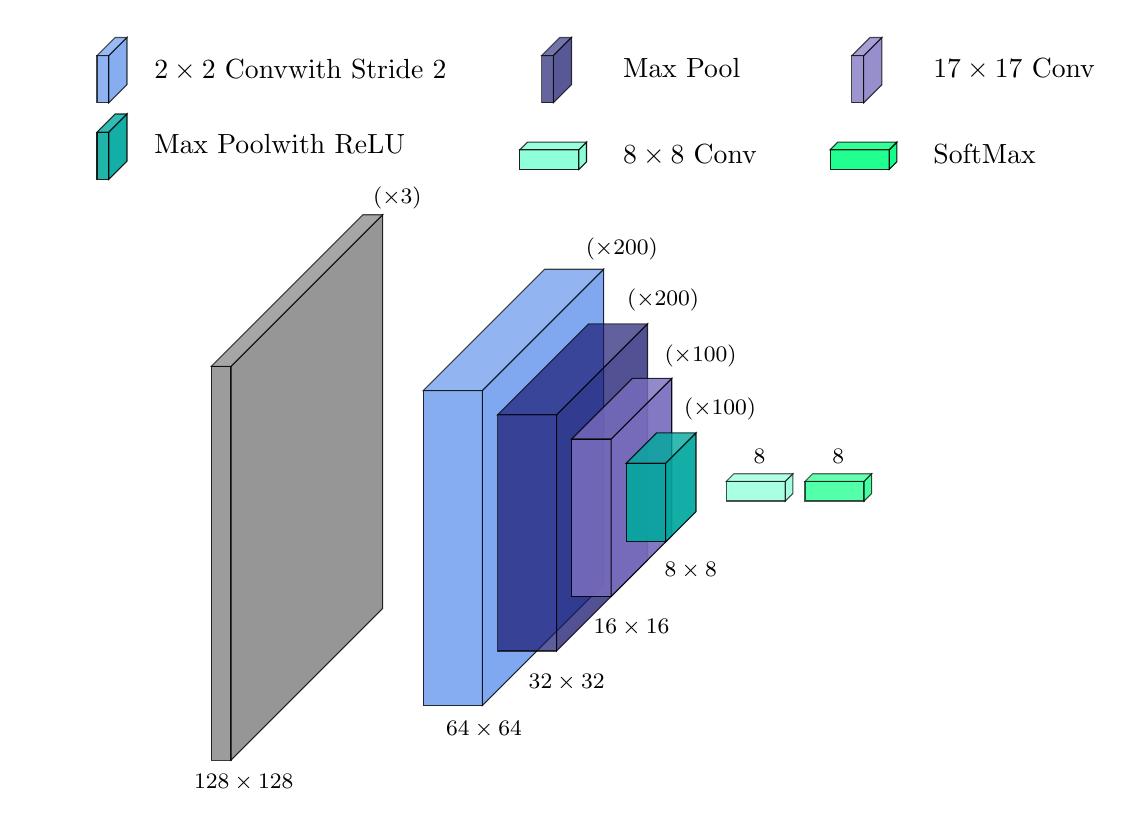
\begin{tikzpicture}[scale=0.5]
  %%%%%%%%%%%%%%%%%%%%%%%%%%%%%%%%%%%%%%%%%%%%%%%%%%%%%%%%%%%%%%%%%%%%%%%%%%%%%%%%%%%%%%%%%%%%%%%%%%%%%%%%%%%%%%%%%%%%%%%%%%
  %%%  PARAMETERS:
  %%%%%%%%%%%%%%%%%%%%%%%%%%%%%%%%%%%%%%%%%%%%%%%%%%%%%%%%%%%%%%%%%%%%%%%%%%%%%%%%%%%%%%%%%%%%%%%%%%%%%%%%%%%%%%%%%%%%%%%%%%

  
  %%% COLOR PALLETE %%%
  \def\colora{CornflowerBlue}
  \def\colorb{Gray}
  \def\colorf{MidnightBlue}
  
  %%% CENTER X-Y COORDINATES
  \def\cx{0}
  \def\cy{0}

  %%% FRONT/SIDE/TOP OPACITIES
  \def\fopac{0.875}
  \def\sopac{0.925}
  \def\topac{0.8}

  \def\fopacb{0.675}
  \def\sopacb{0.725}
  \def\topacb{0.6}


  %%%%%%%%%%%%%%%%%%%%%%%%%%%%
  %%% LEGEND
  %%%%%%%%%%%%%%%%%%%%%%%%%%%%

  %%% CENTER X-Y COORDINATES
  \def\cx{0}
  \def\cy{0}

  \node at (2.25,9.5) {
    \setlength\tabcolsep{1.5pt}
    \begin{tabular}{rlrlrl}
      \def\depth{0.15}
      \def\res{0.3}
      \def\resalt{0.3}
      \def\initd{0}
      \def\fcolor{\colora}
      \tikz{\draw[fill=\fcolor,opacity=0.725] (\initd,\cx-\res,\cy+\resalt) -- ++(\depth,0,0) -- ++(0,2*\res,0) -- ++(-\depth,0,0) -- cycle;
      \draw[fill=\fcolor,opacity=0.775] (\initd+\depth,\cx-\res,\cy+\resalt) -- ++(0,0,-2*\resalt) -- ++(0,2*\res,0) -- ++(0,0,2*\resalt) -- cycle;
      \draw[fill=\fcolor,opacity=0.65] (\initd,\cx+\res,\cy+\resalt) -- ++(\depth,0,0) -- ++(0,0,-2*\resalt) -- ++(-\depth,0,0) -- cycle;}
      & \raisebox{0.125in}{ \hspace{0.0in} \stackanchor{$2\times2$ Conv}{with Stride 2}} \hspace{0.0in}  &
      %%%%%%%%%%%%%%%%%%%%%%%%%%%%%%%%%%%%%%%%%%%%%%%%%%%%%%%%%%%%%%%%%%%%%%%%%%%
      \def\depth{0.15}
      \def\res{0.3}
      \def\resalt{0.3}
      \def\initd{0}
      \def\fcolor{\colorf}
      \tikz{\draw[fill=\fcolor,opacity=\fopacb] (\initd,\cx-\res,\cy+\resalt) -- ++(\depth,0,0) -- ++(0,2*\res,0) -- ++(-\depth,0,0) -- cycle;
      \draw[fill=\fcolor,opacity=\sopacb] (\initd+\depth,\cx-\res,\cy+\resalt) -- ++(0,0,-2*\resalt) -- ++(0,2*\res,0) -- ++(0,0,2*\resalt) -- cycle;
      \draw[fill=\fcolor,opacity=\topacb] (\initd,\cx+\res,\cy+\resalt) -- ++(\depth,0,0) -- ++(0,0,-2*\resalt) -- ++(-\depth,0,0) -- cycle;}
      \hspace{0.075in}
      & \raisebox{0.13in}{ \hspace{0.0in} Max Pool} \hspace{0.0in} &
      %%%%%%%%%%%%%%%%%%%%%%%%%%%%%%%%%%%%%%%%%%%%%%%%%%%%%%%%%%%%%%%%%%%%%%%%%%%
      %%%%%%%%%%%%%%%%%%%%%%%%%%%%%%%%%%%%%%%%%%%%%%%%%%%%%%%%%%%%%%%%%%%%%%%%%%%
      \def\depth{0.15}
      \def\res{0.3}
      \def\resalt{0.3}
      \def\initd{0}
      \def\fcolor{Periwinkle}
      \tikz{\draw[fill=\fcolor,opacity=0.725] (\initd,\cx-\res,\cy+\resalt) -- ++(\depth,0,0) -- ++(0,2*\res,0) -- ++(-\depth,0,0) -- cycle;
      \draw[fill=\fcolor,opacity=0.775] (\initd+\depth,\cx-\res,\cy+\resalt) -- ++(0,0,-2*\resalt) -- ++(0,2*\res,0) -- ++(0,0,2*\resalt) -- cycle;
      \draw[fill=\fcolor,opacity=0.65] (\initd,\cx+\res,\cy+\resalt) -- ++(\depth,0,0) -- ++(0,0,-2*\resalt) -- ++(-\depth,0,0) -- cycle;}
      \hspace{0.075in}
      & \raisebox{0.13in}{ \hspace{0.0in} $17\times17$ Conv} \hspace{0.0in}

      \\
      %%%%%%%%%%%%%%%%%%%%%%%%%%%%%%%%%%%%%%%%%%%%%%%%%%%%%%%%%%%%%%%%%%%%%%%%%%%
      %%%%%%%%%%%%%%%%%%%%%%%%%%%%%%%%%%%%%%%%%%%%%%%%%%%%%%%%%%%%%%%%%%%%%%%%%%%
      \def\depth{0.15}
      \def\res{0.3}
      \def\resalt{0.3}
      \def\initd{0}
      \def\fcolor{Emerald}
      \tikz{\draw[fill=\fcolor,opacity=\fopac] (\initd,\cx-\res,\cy+\resalt) -- ++(\depth,0,0) -- ++(0,2*\res,0) -- ++(-\depth,0,0) -- cycle;
      \draw[fill=\fcolor,opacity=\sopac] (\initd+\depth,\cx-\res,\cy+\resalt) -- ++(0,0,-2*\resalt) -- ++(0,2*\res,0) -- ++(0,0,2*\resalt) -- cycle;
      \draw[fill=\fcolor,opacity=\topac] (\initd,\cx+\res,\cy+\resalt) -- ++(\depth,0,0) -- ++(0,0,-2*\resalt) -- ++(-\depth,0,0) -- cycle;}
      & \raisebox{0.1325in}{ \hspace{0.0in} \stackanchor{Max Pool}{with ReLU}} \hspace{0.0in} &
      %%%%%%%%%%%%%%%%%%%%%%%%%%%%%%%%%%%%%%%%%%%%%%%%%%%%%%%%%%%%%%%%%%%%%%%%%%%
      \raisebox{0.05in}{ 
        \def\depth{0.75}
        \def\res{0.125}
        \def\resalt{0.125}
        \def\initd{0}
        \def\fcolor{Aquamarine}
        \tikz{\draw[fill=\fcolor,opacity=\fopac] (\initd,\cx-\res,\cy+\resalt) -- ++(\depth,0,0) -- ++(0,2*\res,0) -- ++(-\depth,0,0) -- cycle;
          \draw[fill=\fcolor,opacity=\sopac] (\initd+\depth,\cx-\res,\cy+\resalt) -- ++(0,0,-2*\resalt) -- ++(0,2*\res,0) -- ++(0,0,2*\resalt) -- cycle;
          \draw[fill=\fcolor,opacity=\topac] (\initd,\cx+\res,\cy+\resalt) -- ++(\depth,0,0) -- ++(0,0,-2*\resalt) -- ++(-\depth,0,0) -- cycle;}
      }
      & \raisebox{0.0825in}{ \hspace{0.0in} $8\times8$ Conv} \hspace{0.0in} &
      \raisebox{0.05in}{
        %%%%%%%%%%%%%%%%%%%%%%%%%%%%%%%%%%%%%%%%%%%%%%%%%%%%%%%%%%%%%%%%%%%%%%%%%%%
        \def\depth{0.75}
        \def\res{0.125}
        \def\resalt{0.125}
        \def\initd{0}
        \def\fcolor{SpringGreen}
        \tikz{\draw[fill=\fcolor,opacity=\fopac] (\initd,\cx-\res,\cy+\resalt) -- ++(\depth,0,0) -- ++(0,2*\res,0) -- ++(-\depth,0,0) -- cycle;
          \draw[fill=\fcolor,opacity=\sopac] (\initd+\depth,\cx-\res,\cy+\resalt) -- ++(0,0,-2*\resalt) -- ++(0,2*\res,0) -- ++(0,0,2*\resalt) -- cycle;
          \draw[fill=\fcolor,opacity=\topac] (\initd,\cx+\res,\cy+\resalt) -- ++(\depth,0,0) -- ++(0,0,-2*\resalt) -- ++(-\depth,0,0) -- cycle;}
      }
      & \raisebox{0.0825in}{ \hspace{0.0in} SoftMax} \hspace{0.0in} 
      %%%%%%%%%%%%%%%%%%%%%%%%%%%%%%%%%%%%%%%%%%%%%%%%%%%%%%%%%%%%%%%%%%%%%%%%%%%

    \end{tabular}
  };
  

  
  %%%%%%%%%%%%%%%%%%%%%%%%%%%%%%%%%%%%%%%%%%%%%%%%%%%%%%%%%%%%%%%%%%%%%%%%%%%%%%%%%%%%%%%%%%%%%%%%%%%%%%%%%%%%%%%%%%%%%%%%%%
  %%%   LAYERS
  %%%%%%%%%%%%%%%%%%%%%%%%%%%%%%%%%%%%%%%%%%%%%%%%%%%%%%%%%%%%%%%%%%%%%%%%%%%%%%%%%%%%%%%%%%%%%%%%%%%%%%%%%%%%%%%%%%%%%%%%%%
  \def\dfactor{0.25}
  \def\initd{-5}
  \def\depth{0.5}
  \def\res{5}
  \def\fcolor{\colorb}
  %% FRONT
  \draw[fill=\fcolor,opacity=0.775] (\initd,\cx-\res,\cy+\res) -- ++(\depth,0,0) -- ++(0,2*\res,0) -- ++(-\depth,0,0) -- cycle;
  %% SIDE
  \draw[fill=\fcolor,opacity=0.825] (\initd+\depth,\cx-\res,\cy+\res) -- ++(0,0,-2*\res) -- ++(0,2*\res,0) -- ++(0,0,2*\res) -- cycle;
  %% TOP
  \draw[fill=\fcolor,opacity=0.7] (\initd,\cx+\res,\cy+\res) -- ++(\depth,0,0) -- ++(0,0,-2*\res) -- ++(-\depth,0,0) -- cycle;
  \node at (\initd + 2.8,7.35) {\footnotesize$(\times 3)$};
  \node at (\initd + 2-3.1,-7.5) {\footnotesize$128\times128$};

  %%%%%%%%%%%%%%%%%%%%%%%%%%%%%%%%%%%%%%%%%%%%%%%%%%%%%%%%%%%%%%%%%%%%%%%%%%%%%%%%%%%%%%%%%%%%%%%%%%%%%%%%%%%%%%%%%%%%%%%%%%
  \def\dfactor{0.25}
  \def\initd{0}
  \def\depth{1.5}
  \def\res{4}
  \def\fcolor{\colora}
  %% FRONT
  \draw[fill=\fcolor,opacity=0.775] (\initd,\cx-\res,\cy+\res) -- ++(\depth,0,0) -- ++(0,2*\res,0) -- ++(-\depth,0,0) -- cycle;
  %% SIDE
  \draw[fill=\fcolor,opacity=0.825] (\initd+\depth,\cx-\res,\cy+\res) -- ++(0,0,-2*\res) -- ++(0,2*\res,0) -- ++(0,0,2*\res) -- cycle;
  %% TOP
  \draw[fill=\fcolor,opacity=0.7] (\initd,\cx+\res,\cy+\res) -- ++(\depth,0,0) -- ++(0,0,-2*\res) -- ++(-\depth,0,0) -- cycle;
  \node at (\initd + 3.5,6.05) {\footnotesize$(\times 200)$};
  \node at (\initd + 0.0,-6.05-0.1) {\footnotesize$64\times64$};

  %%%%%%%%%%%%%%%%%%%%%%%%%%%%%%%%%%%%%%%%%%%%%%%%%%%%%%%%%%%%%%%%%%%%%%%%%%%%%%%%%%%%%%%%%%%%%%%%%%%%%%%%%%%%%%%%%%%%%%%%%%
  \def\initd{1.5}
  \def\depth{1.5}
  \def\res{3}
  \def\fcolor{\colorf}
  \draw[fill=\fcolor,opacity=0.705] (\initd,\cx-\res,\cy+\res) -- ++(\depth,0,0) -- ++(0,2*\res,0) -- ++(-\depth,0,0) -- cycle;
  \draw[fill=\fcolor,opacity=0.755] (\initd+\depth,\cx-\res,\cy+\res) -- ++(0,0,-2*\res) -- ++(0,2*\res,0) -- ++(0,0,2*\res) -- cycle;
  \draw[fill=\fcolor,opacity=0.685] (\initd,\cx+\res,\cy+\res) -- ++(\depth,0,0) -- ++(0,0,-2*\res) -- ++(-\depth,0,0) -- cycle;
  \node at (4.55,4.75) {\footnotesize$(\times 200)$};
  \node at (3.5-1.4,-4.75-0.2) {\footnotesize$32\times32$};
  %%%%%%%%%%%%%%%%%%%%%%%%%%%%%%%%%%%%%%%%%%%%%%%%%%%%%%%%%%%%%%%%%%%%%%%%%%%%%%%%%%%%%%%%%%%%%%%%%%%%%%%%%%%%%%%%%%%%%%%%%%
  \def\initd{3.0}
  \def\depth{1.0}
  \def\res{2}
  \def\fcolor{Periwinkle}
  \draw[fill=\fcolor,opacity=\fopac] (\initd,\cx-\res,\cy+\res) -- ++(\depth,0,0) -- ++(0,2*\res,0) -- ++(-\depth,0,0) -- cycle;
  \draw[fill=\fcolor,opacity=\sopac] (\initd+\depth,\cx-\res,\cy+\res) -- ++(0,0,-2*\res) -- ++(0,2*\res,0) -- ++(0,0,2*\res) -- cycle;
  \draw[fill=\fcolor,opacity=\topac] (\initd,\cx+\res,\cy+\res) -- ++(\depth,0,0) -- ++(0,0,-2*\res) -- ++(-\depth,0,0) -- cycle;
  \node at (5.5,3.35) {\footnotesize$(\times 100)$};
  \node at (4.75-1.0,-3.5-0.05) {\footnotesize$16\times16$};


  %%%%%%%%%%%%%%%%%%%%%%%%%%%%%%%%%%%%%%%%%%%%%%%%%%%%%%%%%%%%%%%%%%%%%%%%%%%%%%%%%%%%%%%%%%%%%%%%%%%%%%%%%%%%%%%%%%%%%%%%%%



  
  %%%%%%%%%%%%%%%%%%%%%%%%%%%%%%%%%%%%%%%%%%%%%%%%%%%%%%%%%%%%%%%%%%%%%%%%%%%%%%%%%%%%%%%%%%%%%%%%%%%%%%%%%%%%%%%%%%%%%%%%%%
  \def\initd{4.0}
  \def\depth{1.0}
  \def\res{1}
  \def\fcolor{Emerald}
  \draw[fill=\fcolor,opacity=\fopac] (\initd,\cx-\res,\cy+\res) -- ++(\depth,0,0) -- ++(0,2*\res,0) -- ++(-\depth,0,0) -- cycle;
  \draw[fill=\fcolor,opacity=\sopac] (\initd+\depth,\cx-\res,\cy+\res) -- ++(0,0,-2*\res) -- ++(0,2*\res,0) -- ++(0,0,2*\res) -- cycle;
  \draw[fill=\fcolor,opacity=\topac] (\initd,\cx+\res,\cy+\res) -- ++(\depth,0,0) -- ++(0,0,-2*\res) -- ++(-\depth,0,0) -- cycle;
  \node at (6.0,2.0) {\footnotesize$(\times 100)$};
  \node at (5.25,-2.0-0.1) {\footnotesize$8\times8$};
  %%%%%%%%%%%%%%%%%%%%%%%%%%%%%%%%%%%%%%%%%%%%%%%%%%%%%%%%%%%%%%%%%%%%%%%%%%%%%%%%%%%%%%%%%%%%%%%%%%%%%%%%%%%%%%%%%%%%%%%%%%


  
  %%%%%%%%%%%%%%%%%%%%%%%%%%%%%%%%%%%%%%%%%%%%%%%%%%%%%%%%%%%%%%%%%%%%%%%%%%%%%%%%%%%%%%%%%%%%%%%%%%%%%%%%%%%%%%%%%%%%%%%%%%
  %%%    FULLY CONNECTED
  %%%%%%%%%%%%%%%%%%%%%%%%%%%%%%%%%%%%%%%%%%%%%%%%%%%%%%%%%%%%%%%%%%%%%%%%%%%%%%%%%%%%%%%%%%%%%%%%%%%%%%%%%%%%%%%%%%%%%%%%%%
  %%%%%%%%%%%%%%%%%%%%%%%%%%%%%%%%%%%%%%%%%%%%%%%%%%%%%%%%%%%%%%%%%%%%%%%%%%%%%%%%%%%%%%%%%%%%%%%%%%%%%%%%%%%%%%%%%%%%%%%%%%
  \def\centerdepth{4.0}
  \def\initd{\centerdepth+2.25}
  \def\depth{1.5}
  \def\resx{0.25}
  \def\resy{0.25}
  \def\fcolor{Aquamarine}
  \draw[fill=\fcolor,opacity=\fopacb] (\initd,\cx-\resx,\cy+\resy) -- ++(\depth,0,0) -- ++(0,2*\resx,0) -- ++(-\depth,0,0) -- cycle;
  \draw[fill=\fcolor,opacity=\sopacb] (\initd+\depth,\cx-\resx,\cy+\resy) -- ++(0,0,-2*\resy) -- ++(0,2*\resx,0) -- ++(0,0,2*\resy) -- cycle;
  \draw[fill=\fcolor,opacity=\topacb] (\initd,\cx+\resx,\cy+\resy) -- ++(\depth,0,0) -- ++(0,0,-2*\resy) -- ++(-\depth,0,0) -- cycle;
  \node at (\centerdepth+3.0,0.8) {\footnotesize$8$};
  %%%%%%%%%%%%%%%%%%%%%%%%%%%%%%%%%%%%%%%%%%%%%%%%%%%%%%%%%%%%%%%%%%%%%%%%%%%%%%%%%%%%%%%%%%%%%%%%%%%%%%%%%%%%%%%%%%%%%%%%%%

  \def\centerdepth{6.0}
  \def\initd{\centerdepth+2.25}
  \def\depth{1.5}
  \def\resx{0.25}
  \def\resy{0.25}
  \def\fcolor{SpringGreen}
  \draw[fill=\fcolor,opacity=\fopacb] (\initd,\cx-\resx,\cy+\resy) -- ++(\depth,0,0) -- ++(0,2*\resx,0) -- ++(-\depth,0,0) -- cycle;
  \draw[fill=\fcolor,opacity=\sopacb] (\initd+\depth,\cx-\resx,\cy+\resy) -- ++(0,0,-2*\resy) -- ++(0,2*\resx,0) -- ++(0,0,2*\resy) -- cycle;
  \draw[fill=\fcolor,opacity=\topacb] (\initd,\cx+\resx,\cy+\resy) -- ++(\depth,0,0) -- ++(0,0,-2*\resy) -- ++(-\depth,0,0) -- cycle;
  \node at (\centerdepth+3.0,0.8) {\footnotesize$8$};
  %%%%%%%%%%%%%%%%%%%%%%%%%%%%%%%%%%%%%%%%%%%%%%%%%%%%%%%%%%%%%%%%%%%%%%%%%%%%%%%%%%%%%%%%%%%%%%%%%%%%%%%%%%%%%%%%%%%%%%%%%%

  % Lines connecting conv layers to dense layers
  %\draw[dashed] (\centerdepth+1.15,0,0) -- (\centerdepth+1.9,0,0);
  %\draw[dashed] (\centerdepth+1.15,0.25,0) -- (\centerdepth+1.9,2.0,0);
  %\draw[dashed] (\centerdepth+1.15,-0.25,0) -- (\centerdepth+1.9,-2.0,0);

\end{tikzpicture}
\end{center}





\end{document}
